\documentclass[11pt]{article}

\ProvidesPackage{sammath}

% Math stuff
\usepackage{epsfig}
\usepackage{amsfonts}
\usepackage{amssymb}
\usepackage{amstext}
\usepackage{amsmath}
\usepackage{bbm}
\usepackage{bm}
\usepackage{centernot}
\usepackage{mathtools}
\usepackage{xcolor,colortbl}
\usepackage{units}

% Graphics
\usepackage{xspace}
\usepackage{graphicx}
\usepackage{tikz}

% Symbols (must be before math stuff) to no override math symbols
\let\oldint\int
\let\oldiint\iint
\let\oldiiint\iiint

\usepackage{wasysym}
\usepackage{marvosym}

\let\int\oldint
\let\iint\oldiint
\let\iiint\oldiiint

% Replace all astericks with \cdot
\DeclareMathSymbol{*}{\mathbin}{symbols}{"01}

% Figures and Tables
\usepackage[center]{caption}
\usepackage{subfig}
\usepackage{longtable}
			
\newcommand*{\tabvpad}[1]{\def\arraystretch{#1}}
\newcommand*{\tabhpad}[1]{\setlength{\tabcolsep}{#1}}

% Enumerators
\usepackage[shortlabels]{enumitem}

% For tables
\usepackage{tabularx}
\usepackage{booktabs}

% ECE
\usepackage{karnaugh-map}
\usepackage{svg}

% Venn Diagrams
\newcommand{\vertex}{\node[vertex]}
\tikzstyle{vertex}=[circle,fill=black!20]

% This is the stuff for normal spacing
\makeatletter
\setlength{\textwidth}{6in}
\setlength{\oddsidemargin}{0in}
\setlength{\evensidemargin}{0.5in}
\setlength{\topmargin}{0in}
\setlength{\textheight}{8.5in}
\setlength{\headheight}{0pt}
\setlength{\headsep}{0pt}
% \setlength{\marginparwidth}{59pt}
\setlength{\marginparwidth}{0pt}
\setlength{\marginparsep}{0pt}

\setlength{\parindent}{0pt}
\setlength{\parskip}{5pt plus 1pt}

\newtheorem{theorem}{Theorem}
\newtheorem{lemma}[theorem]{Lemma}
\newtheorem{proposition}[theorem]{Proposition}
\newtheorem{claim}[theorem]{Claim}
\newtheorem{corollary}[theorem]{Corollary}
\newtheorem{definition}[theorem]{Definition}

% Proof Environment
\newcommand{\proofbox}{\hfill\ensuremath{\square}}
\newenvironment{proof}{{ \bf Proof:  }}{\proofbox}

\newenvironment{proofby}[1]{{\bf Proof (by #1):  }}{\proofbox}
\newenvironment{proofbynobrackets}[1]{{\bf Proof by #1:  }}{\proofbox}
\newenvironment{proofbyMI}[1]{{\bf Proof (by induction):  }}{\proofbox}
\newenvironment{proofbyinduction}{{\bf Proof (by induction):  }}{\proofbox}
\newenvironment{proofbystronginduction}{{\bf Proof (by strong induction):  }}{\proofbox}
\newenvironment{proofbycontradiction}{{\bf Proof (by contradiction):  }}{\proofbox}
\newenvironment{proofbycontrapositive}{{\bf Proof (by contrapositive):  }}{\proofbox}

\newenvironment{proofof}[1]{{\bf Proof of #1:  }}{\proofbox}
\newenvironment{proofofnobox}[1]{{\bf#1:  }}{}

\newenvironment{example}{{\bf Example:  }}{\proofbox}

% Math Notation
\newcommand*{\R}{\ensuremath{\mathbb R}}
\newcommand*{\Z}{\ensuremath{\mathbb Z}}
\newcommand*{\N}{\ensuremath{\mathbb N}}
\newcommand*{\Q}{\ensuremath{\mathbb Q}}
\newcommand*{\B}{\ensuremath{\mathbb B}}

%% True False
\newcommand*{\T}{\ensuremath{\checkmark}}
% \newcommand*{\F}{\ensuremath{\times}}
\newcommand*{\contradiction}{\Rightarrow\Leftarrow}

%% Text Formatting
\newcommand*{\suchthat}{\text{\ \ s.t. }}
\newcommand*{\st}{\suchthat}
\newcommand*{\textand}{\text{ and }}

\newcommand*{\LHS}{\text{LHS}}
\newcommand*{\RHS}{\text{RHS}}

\newcommand{\simpleheader}[1]{\underline{\textit{#1:}}\quad\ \vspace{0.1in} }
\newcommand{\simpleheaderln}[1]{\simpleheader{#1} \\ }
\newcommand{\littleheader}[2]{\underline{\textit{#1: #2}} \vspace{0.1in} \\ }
\newcommand{\WTS}[1]{\littleheader{WTS}{#1}}
\newcommand{\WTF}[1]{\littleheader{WTF}{#1}}
\newcommand{\case}[2]{\littleheader{Case #1}{#2}}

\newcommand{\venntitle}[1]{\ensuremath{\underline{#1}} \\ \\}

\newcommand*{\quador}{\quad\text{or}\quad}
\newcommand*{\quadand}{\quad\text{and}\quad}

\newcommand*{\bezoutslemma}{\text{B\'ezout's Lemma}}
\newcommand{\annotate}[1]{&& \left(\text{#1}\right)}
\newcommand{\annotateln}[1]{\annotate{#1} \\}
\newcommand{\annotatefracln}[1]{\annotate{#1} \fracln}

%% Other formating
\newcommand*{\notimplies}{\ensuremath{\centernot \implies}}
\newcommand*{\notimpliedby}{\ensuremath{\centernot \impliedby}}
\newcommand*{\forwarddirection}{(\ensuremath{ \implies })\qquad}
\newcommand*{\reversedirection}{(\ensuremath{ \impliedby })\qquad}
\newcommand{\vecln}{\\[0.75ex]}
\newcommand{\fracln}{\\[1.5ex]}

\newcommand*{\ceil}[1]{\ensuremath{\left\lceil #1 \right\rceil}}
\newcommand*{\floor}[1]{\ensuremath{\left\lfloor #1 \right\rfloor}}
\newcommand*{\abs}[1]{\ensuremath{\left|#1\right|}}
\newcommand*{\abss}[1]{\abs{#1 \strut}}
\newcommand*{\absstrut}[1]{\abss{#1}}

%% Sets
\newcommand*{\powerset}[1]{\ensuremath{\mathcal{P}(#1)}}
\newcommand*{\set}[1]{\ensuremath{\left\{#1\right\}}}
\newcommand*{\union}{\ensuremath{\cup}}
\newcommand*{\intersect}{\ensuremath{\cap}}
\newcommand*{\setst}{\ensuremath{\ \middle|\ }}
\newcommand*{\plainsetst}{\ |\ }

\let\oldemptyset\emptyset
\let\emptyset\varnothing

%% Functions 
\newcommand{\id}[2]{\text{id}_{#1}(#2)}
\newcommand*{\inverse}[1]{\ensuremath{#1^{-1}}}
\newcommand*{\inversep}[1]{\ensuremath{\left(#1\right)^{-1}}}
\newcommand*{\inverseb}[1]{\ensuremath{\left[#1\right]^{-1}}}
\newcommand*{\composite}{\ensuremath{\circ}}

%% Divisibility and GCD Stuff
\newcommand*{\coprime}{\ensuremath{\ \perp\ }}
\newcommand*{\notcoprime}{\ensuremath{\ \not\perp\ }}
\newcommand*{\divides}{\ensuremath{\ \mid\ }}
\newcommand*{\notdivides}{\ensuremath{\nmid}}
\newcommand*{\congruent}{\ensuremath{\equiv}}
\newcommand*{\lcm}{\text{lcm}}
\newcommand*{\totient}[1]{\ensuremath{\varphi(#1)}}

%% Induction
\newcommand*{\IH}{\text{I.H.}}
\newcommand*{\SIH}{\text{S.I.H.}}
\newcommand*{\basecase}{\simpleheader{Base Case}}
\newcommand*{\basecases}{\simpleheader{Base Cases}}
\newcommand*{\inductivestep}{\simpleheader{Inductive Step}}
\newcommand*{\inductivecase}{\inductivestep}
\newcommand*{\propP}[1]{P\ensuremath{(#1)}}
\newcommand{\ptrue}[1]{\propP{#1} \text{is true}}
\newcommand{\inductionconclusion}[3]{Therefore, since \ptrue{#1}, and #3, \ptrue{#2} \ensuremath{\implies} \ptrue{#2+1}, by mathematical induction, the proposition \ptrue{#2} #3.}
%\newcommand{\stronginductionconclusion}[4]{Therefore, since \ptrue{#1}, and for all $n\geq #1$ #2, [,$ \forall #1 \leq $ \ptrue{#3}$ ] \implies $ \ptrue{#2+1}, by mathematical induction, the proposition \ptrue{#2} #3.}

%% Diff Eq
\newcommand*{\pif}[1]{\ensuremath{\frac{\pi}{#1}}}
\newcommand*{\dpif}[1]{\ensuremath{\displaystyle\pif{#1}}}
\newcommand*{\ddp}[2]{\ensuremath{\dfrac{\partial#1}{\partial#2}}} % partial derv
\newcommand*{\ddf}[2]{\ensuremath{\dfrac{{d}#1}{{d}#2}}}
\newcommand*{\dydx}{\ensuremath{\ddf{y}{x}}}
\newcommand*{\dydt}{\ensuremath{\ddf{y}{t}}}
\newcommand*{\wrt}[1]{\ensuremath{\text{with respect to }#1}}
\newcommand*{\diffeq}{\text{differential equation}}
\newcommand*{\derv}[1]{\ensuremath{\cdot d#1}}
\newcommand*{\du}{\derv{u}}
\newcommand*{\dx}{\derv{x}}
\newcommand*{\dy}{\derv{y}}
\newcommand*{\dt}{\derv{t}}
\newcommand*{\dv}{\derv{v}}
\newcommand*{\dtau}{\derv{\tau}}
\newcommand*{\domega}{\derv{\omega}}
\newcommand*{\dOmega}{\derv{\Omega}}
\newcommand*{\dw}{\domega}
\newcommand*{\dW}{\dOmega}


\newcommand*{\intinfty}{\int_{-\infty}^{\infty}}
\newcommand*{\intzeroinfty}{\int_{0}^{\infty}}
\newcommand*{\suminfty}[1]{\sum_{#1 = -\infty}^{\infty}}
\newcommand*{\sumzeroinfty}[1]{\sum_{#1 = 0}^{\infty}}

\newcommand{\bunderline}[2][4]{\underline{#2\mkern-#1mu}\mkern#1mu }
\newcommand*{\uv}[1]{\bunderline{\ensuremath{#1}}}
\newcommand*{\uvec}[1]{\uv{#1}}

\def\vv{\ensuremath{\vec{\bf v}}}
\def\vva{\ensuremath{\vv_1}}
\def\vvb{\ensuremath{\vv_2}}

\usepackage[scr]{rsfso}
\newcommand*{\Laplacesymbol}{\ensuremath{\mathscr{L}}}
\newcommand*{\Laplace}[1]{\ensuremath{\Laplacesymbol\left\{#1\right\}}}
\newcommand*{\LaplaceInv}[1]{\ensuremath{\inverse{\Laplacesymbol}\left\{#1\right\}}}
\newcommand*{\Lapl}[1]{\ensuremath{\Laplace{#1}}}
\newcommand*{\LaplInv}[1]{\ensuremath{\LaplaceInv{#1}}}
\newcommand*{\LaplaceInverse}[1]{\ensuremath{\LaplaceInv{#1}}}

\newcommand*{\Fouriersymbol}{\mathcal{F}}
\newcommand*{\FT}[1]{\ensuremath{\Fouriersymbol\left\{#1\right\}}}
\newcommand*{\FTInv}[1]{\ensuremath{\inverse{\Fouriersymbol}\left\{#1\right\}}}
\newcommand*{\FTarrow}[1]{\quad\xleftrightarrow{\text{ #1 }}\quad}

\newcommand*{\LaplaceArrow}{\FTarrow{\Laplacesymbol}}
\newcommand*{\LaplArrow}{\LaplaceArrow}

\newcommand*{\CTFT}{\FTarrow{CTFT}}
\newcommand*{\CTFS}{\FTarrow{CTFS, \ensuremath{\omega_0}}}

\newcommand*{\DTFT}{\FTarrow{DTFT}}
\newcommand*{\DTFS}{\FTarrow{DTFS, \ensuremath{\Omega_0}}}

% 18-290 stuff
\newcommand*{\system}[1]{\ensuremath{\mathcal{H}\set{#1}}}
\newcommand*{\conv}{\ensuremath{\ast}}
\newcommand*{\circconv}{\ensuremath{\circledast}}

\def\jomega{\ensuremath{j \omega}}
\def\jw{\jomega}

\def\jOmega{\ensuremath{j \Omega}}
\def\jW{\jOmega}

\makeatletter
\newcommand{\Xjw}[1][\@nil]{
	\def\tmp{#1}%
   	\ifx\tmp\@nnil
		\ensuremath{\ensuremath{X(\jomega)}}
    \else
		\ensuremath{\ensuremath{X_{#1}(\jomega)}}
    \fi
}

\newcommand{\Yjw}[1][\@nil]{
	\def\tmp{#1}%
   	\ifx\tmp\@nnil
		\ensuremath{\ensuremath{Y(\jomega)}}
    \else
		\ensuremath{\ensuremath{Y_{#1}(\jomega)}}
    \fi
}

\newcommand{\Hjw}[1][\@nil]{
	\def\tmp{#1}%
   	\ifx\tmp\@nnil
		\ensuremath{\ensuremath{H(\jomega)}}
    \else
		\ensuremath{\ensuremath{H_{#1}(\jomega)}}
    \fi
}
\makeatother

\def\Xjomega{\Xjw}
\def\Yjomega{\Yjw}
\def\Hjomega{\Hjw}

\makeatletter
\newcommand{\XejW}[1][\@nil]{
	\def\tmp{#1}%
   	\ifx\tmp\@nnil
		\ensuremath{X(e^{\jOmega})}
    \else
		\ensuremath{X_{#1}(e^{\jOmega})}
    \fi
}

\newcommand{\YejW}[1][\@nil]{
	\def\tmp{#1}%
   	\ifx\tmp\@nnil
		\ensuremath{Y(e^{\jOmega})}
    \else
		\ensuremath{Y_{#1}(e^{\jOmega})}
    \fi
}

\newcommand{\HejW}[1][\@nil]{
	\def\tmp{#1}%
   	\ifx\tmp\@nnil
		\ensuremath{H(e^{\jOmega})}
    \else
		\ensuremath{H_{#1}(e^{\jOmega})}
    \fi
}

\makeatother

\def\XejOmega{\XejW}
\def\YejOmega{\YejW}
\def\HejOmega{\HejW}

\newcommand*{\conj}[1]{\ensuremath{{#1}^{\ast}}}
\newcommand*{\conjugate}[1]{\conj{#1}}

\newcommand*{\sinc}{\mathrm{sinc}}

\newcommand*{\stepfn}[1]{\mathscr{U}\left(#1\right)}

\newcommand{\mnote}[1]{\normalmarginpar \marginpar{\tiny #1}}
\newcommand{\junk}[1]{}

\newenvironment{sol}{
	\textbf{Solution:}
}

\def\ws{\ensuremath{\omega_s}}
\def\wm{\ensuremath{\omega_m}}
\def\wc{\ensuremath{\omega_c}}
\def\wo{\ensuremath{\omega_0}}
\def\wl{\ensuremath{\omega_\ell}}
\def\wh{\ensuremath{\omega_h}}

%% ECE Stuffs
\newcommand*{\xor}{\ensuremath{\oplus}}
\newcommand*{\enot}[1]{\ensuremath{\overline{#1\strut}}}

%% Robotics Stuffs
\newcommand*{\Lagrange}{\ensuremath{\mathcal{L}}}

%% dots{}
\newcommand*{\dotx}{\ensuremath{\dot{x}}}
\newcommand*{\doty}{\ensuremath{\dot{y}}}
\newcommand*{\dotq}{\ensuremath{\dot{q}}}
\newcommand*{\dottheta}{\ensuremath{\dot{\theta}}}

\newcommand*{\dotth}{\dottheta}
\newcommand*{\thdot}{\dottheta}
\newcommand*{\thetadot}{\dottheta}
\newcommand*{\xdot}{\dotx}
\newcommand*{\ydot}{\doty}
\newcommand*{\qdot}{\dotq}

%% ddots{}
\newcommand*{\thetaddot}{\ensuremath{\ddot{\theta}}}
\newcommand*{\xddot}{\ensuremath{\ddot{x}}}
\newcommand*{\yddot}{\ensuremath{\ddot{y}}}
\newcommand*{\qddot}{\ensuremath{\ddot{q}}}

\newcommand*{\ddotx}{\xddot}
\newcommand*{\ddoty}{\yddot}
\newcommand*{\ddotq}{\qddot}
\newcommand*{\ddottheta}{\thetaddot}

% Controls Stuff
\def\mB{{\bf B}}
\def\mC{{\bf C}}
\def\mD{{\bf D}}

\newcommand*{\observemat}{\ensuremath{\mathcal{O}}}
\newcommand*{\controlmat}{\ensuremath{\mathcal{C}}}
\newcommand*{\controllabilitymatrix}{\controlmat}

%%%%%%%%%%%%%%%%%%%%%%%%%%%%%%%%%%%%%%%%%%%%%%%%%%%%%%%
% BOLD ALIGN
%%%%%%%%%%%%%%%%%%%%%%%%%%%%%%%%%%%%%%%%%%%%%%%%%%%%%%%

\usepackage{etoolbox}
\usepackage{environ}

\makeatletter
\NewEnviron{balign*}{%
	\appto\@lign{\balign@row}%
	\gdef\balign@row{\mathversion{normal}}%
	\begin{align*}
		\BODY
	\end{align*}
}
\newcommand{\normalrow}{%
	\noalign{\gdef\balign@row{\mathversion{normal}}}%
}
\newcommand{\boldrow}{
	\noalign{\gdef\balign@row{\mathversion{bold}}}%
}
\makeatother

%%%%%%%%%%%%%%%%%%%%%%%%%%%%%%%%%%%%%%%%

%%%%%%%%%%%%%%%%%%%%%%%%%%%%%%%%%%%%%%%%%%%%%
% CENTER FLOAT (CENTERING OVERFLOW IMAGES)
%%%%%%%%%%%%%%%%%%%%%%%%%%%%%%%%%%%%%%%%%%%%%

\makeatletter
\newcommand*{\centerfloat}{%
	\parindent \z@
	\leftskip \z@ \@plus 1fil \@minus \textwidth
	\rightskip\leftskip
	\parfillskip \z@skip}
\makeatother

%%%%%%%%%%%%%%%%%%%%%%%%%%%%%%%%%%%%%

% Big dot
\makeatletter
\newcommand*{\bigcdot}{}% Check if undefined
\DeclareRobustCommand*{\bigcdot}{%
  \mathbin{\mathpalette\bigcdot@{}}%
}
\newcommand*{\bigcdot@scalefactor}{.6}
\newcommand*{\bigcdot@widthfactor}{1.15}
\newcommand*{\bigcdot@}[2]{%
  % #1: math style
  % #2: unused
  \sbox0{$#1\vcenter{}$}% math axis
  \sbox2{$#1\cdot\m@th$}%
  \hbox to \bigcdot@widthfactor\wd2{%
    \hfil
    \raise\ht0\hbox{%
      \scalebox{\bigcdot@scalefactor}{%
        \lower\ht0\hbox{$#1\bullet\m@th$}%
      }%
    }%
    \hfil
  }%
}
\makeatother

%% Argmax and argmin
\DeclareMathOperator*{\argmin}{argmin}   % Jan Hlavacek
\DeclareMathOperator*{\argmax}{argmax}   % Jan Hlavacek

%% Optimisation
\newcommand*{\domain}{\ensuremath{\mathrm{dom}}}
\newcommand*{\dom}{\domain}
\newcommand*{\curlylt}{\ensuremath{\prec}}
\newcommand*{\curlyleq}{\ensuremath{\preceq}}
\newcommand*{\curlygt}{\ensuremath{\succ}}
\newcommand*{\curlygeq}{\ensuremath{\succeq}}
\newcommand*{\indicator}{\ensuremath{\mathbbm{1}}}
\newcommand*{\xstar}{\ensuremath{x^\ast}}
\newcommand*{\lambdastar}{\ensuremath{\lambda^\ast}}
\newcommand*{\nustar}{\ensuremath{\nu^\ast}}
\newcommand*{\vxstar}{\ensuremath{\vx^\ast}}
\newcommand*{\vlambdastar}{\ensuremath{\vlambda^\ast}}
\newcommand*{\vnustar}{\ensuremath{\vnu^\ast}}

%% Probability and Stats
\newcommand*{\prob}[1]{\ensuremath{P\left(#1\right)}}
\newcommand*{\given}{\plainsetst}
\newcommand*{\tallgiven}{\setst}
\newcommand*{\otherwise}{0 & \text{otherwise}}
\newcommand*{\iid}{\ensuremath{\stackrel{\text{\tiny iid}}{\sim}}}
\newcommand*{\expected}[1]{\ensuremath{\mathbb{E}\left[#1\right]}}
\newcommand*{\variance}[1]{\text{Var}\left[#1\right]}
\newcommand*{\ybar}{\ensuremath{\bar{y}}}
\newcommand*{\Ybar}{\ensuremath{\enot{Y}}}
\newcommand*{\bary}{\ybar}
\newcommand*{\barY}{\Ybar}
\newcommand*{\condind}{\mathrel{\text{\scalebox{1.07}{\ensuremath{\perp\mkern-10mu\perp}}}}}
\newcommand*{\condindep}{\condind}
\newcommand*{\from}{\leftarrow}
\newcommand*{\tofro}{\leftrightarrow}
\newcommand*{\tofrom}{\tofro}

\newcommand*{\dth}{\ensuremath{\dot\theta}}
\newcommand*{\htheta}{\ensuremath{\hat{\theta}}}
\newcommand*{\thetahat}{\htheta}
\newcommand*{\valpha}{\ensuremath{\boldsymbol{\alpha}}}
\newcommand*{\vbeta}{\ensuremath{\boldsymbol{\beta}}}
\newcommand*{\vhbeta}{\ensuremath{\boldsymbol{\hat{\beta}}}}
\newcommand*{\vbetahat}{\vhbeta}

\newcommand*{\sumn}[1][i]{\ensuremath{\sum^{n}_{#1=1}}}
\newcommand*{\prodn}[1][i]{\ensuremath{\prod^{n}_{#1=1}}}
\newcommand*{\dsumn}[1][i]{\ensuremath{\displaystyle\sumn[#1]}}
\newcommand*{\dprodn}[1][i]{\ensuremath{\displaystyle\prodn[#1]}}
\newcommand*{\nlist}[2][n]{\ensuremath{{#2}_{1}, \dots, {#2}_{#1}}}

%% Computer Vision
%%% Matrices stuff and formatting
\def\dash{\text{ --- }}
\newcommand{\rank}{\ensuremath{\mathrm{rank}}}
\newcommand{\col}{\ensuremath{\mathrm{col}}}
\newcommand{\trace}{\ensuremath{\mathrm{trace}}}

\newcommand*{\transsymb}{\ensuremath{\top}}
\newcommand*{\transpose}[1]{\ensuremath{{#1}^{\transsymb}}}
\newcommand*{\trans}[1]{\transpose{#1}}
\newcommand*{\transp}[1]{\transpose{\left(#1\right)}}
\newcommand*{\transb}[1]{\transpose{\left[#1\right]}}

\newcommand{\bmat}[1]{\ensuremath{\begin{bmatrix}#1\end{bmatrix}}}
\newcommand{\bbmat}[1]{\begingroup \boldmath \bmat{#1} \endgroup}

\newcommand{\transbmat}[1]{\trans{\bmat{#1}}}
\newcommand{\inversebmat}[1]{\inverse{\bmat{#1}}}
\newcommand{\transbbmat}[1]{\trans{\bbmat{#1}}}
\newcommand{\inversebbmat}[1]{\inverse{\bbmat{#1}}}

\def\vO{{\bf 0}}
\def\zerovec{\ensuremath{\vec{\vO}}}

\def\vp{{\bf p}}
\def\vu{{\bf u}}
\def\vx{{\bf x}}
\def\vxa{\ensuremath{\vx_\mathbf{1}}}
\def\vxb{\ensuremath{\vx_\mathbf{2}}}
\def\vy{{\bf y}}
\def\vt{{\bf t}}
\def\vl{{\bm{\ell}}}
\def\ve{{\bf e}}
\def\vea{{\ve_\mathbf{1}}}
\def\veb{{\ve_\mathbf{2}}}
\def\vh{{\bf h}}
\def\vs{{\bf s}}
\def\vz{{\bf z}}
\def\vw{{\bf w}}
\def\vmu{\ensuremath{\boldsymbol{\mu}}}
\def\vlambda{\ensuremath{\boldsymbol{\lambda}}}
\def\vnu{\ensuremath{\boldsymbol{\nu}}}

\def\vm{{\bf m}}
\def\vc{{\bf c}}
\def\vb{{\bf b}}
\def\vd{{\bf d}}
\def\vq{{\bf q}}
\def\vX{{\bf X}}
\def\mH{{\bf H}}
\def\mA{{\bf A}}
\def\mM{{\bf M}}
\def\mR{{\bf R}}
\def\mT{{\bf T}}
\def\mE{{\bf E}}
\def\mF{{\bf F}}

\def\mP{{\bf P}}
\def\mPa{\ensuremath{\mP_\mathbf{1}}}
\def\mPb{\ensuremath{\mP_\mathbf{2}}}

\def\mK{{\bf K}}
\def\mKa{\ensuremath{\mK_\mathbf{1}}}
\def\mKb{\ensuremath{\mK_\mathbf{2}}}

\def\mI{{\bf I}}

\def\bW{{\bf W}}
\def\mJ{{\bf J}}
\def\del{\ensuremath{\vec{\nabla}}}

\def\tx{\ensuremath{\tilde{\bf x}}}
\def\ta{\ensuremath{\tilde{\bf a}}}
\def\tb{\ensuremath{\tilde{\bf b}}}
\def\tc{\ensuremath{\tilde{\bf c}}}
\def\hn{\ensuremath{\bf \hat{n}}}
\def\hv{\ensuremath{\bf \hat{v}}}
\def\hh{\ensuremath{\bf \hat{h}}}
\def\hs{\ensuremath{\bf \hat{s}}}

\newcommand*{\F}[1]{\ensuremath{\mathcal{F}\left\{#1\right\}}} % fourier transform
\newcommand*{\norm}[1]{\ensuremath{\left\lVert#1\right\rVert}}

\renewcommand{\Re}[1]{\ensuremath{\operatorname{Re}\left\{#1\right\}}}
\renewcommand{\Im}[1]{\ensuremath{\operatorname{Im}\left\{#1\right\}}}

\newcommand*{\vstrut}{\vphantom{\enot{A}}}

% For equation counters
\newcommand*{\stepeqn}{\stepcounter{equation}}
\newcommand*{\stepequation}{\stepeqn}
\newcommand*{\tageqn}{\tag{\theequation}}
\newcommand*{\tagequation}{\tageqn}
\newcommand*{\steptageqn}{\stepeqn\tageqn}
\newcommand*{\steptagequation}{\steptageqn}

%%%%%%%%%%%%%%%%%%%%%%%%%%%%%%%%%%%%%%%%%%%%%%%%%%%%%
% Heading Information
%%%%%%%%%%%%%%%%%%%%%%%%%%%%%%%%%%%%%%%%%%%%%%%%%%%%

\newcommand{\myname}{Samuel Leong Chee Weng}
\newcommand{\myandrew}{\textit{scleong}}

\newcommand{\assignmenttype}{Homework} % homework by default
\newcommand{\headings}{
	\large{\textbf{\mycourse \hfill \assignmenttype\ \myhwnum} \\
		\textbf{\myname \hfill \myandrew}}
	\rule[0.1in]{\textwidth}{0.01in}
}

\newcommand{\headingbreak}{\pagebreak\headings}

\newcommand{\partnername}{My Partner}
\newcommand{\partnerandrew}{\textit{My Partner}}

\newcommand{\headingsshared}{
	\large{\textbf{\mycourse \hfill \assignmenttype\ \myhwnum} \\
		\textbf{\myname \hfill \myandrew} \\ 
		\textbf{\partnername \hfill \partnerandrew }}
	\rule[0.1in]{\textwidth}{0.01in}
}

%%%%%%%%%%%%%%%%%%%%%%%%%%%%%%%%%%%%%%%%%%%%%%%%%%%%%
% New question environment
%%%%%%%%%%%%%%%%%%%%%%%%%%%%%%%%%%%%%%%%%%%%%%%%%%%%
\newcounter{questioncounter}

% For skipping questions
\newcommand*{\skipquestion}{\stepcounter{questioncounter}}

% Problem by default; Use \renewcommand to change to something like "Question" or "Task"
\newcommand*{\questiontype}{Problem} 
\newcommand{\questionhdr}[2][]{\vspace{0.7em} \hrule\vspace{0.5em}
	\noindent{\bf \questiontype\ #2: #1} \vspace{0.5em}
	\hrule}

% For resuming counter for question part
\newcounter{questionpartcounter}
\newcommand*{\setquestioncount}[1]{\setcounter{questioncounter}{#1}}
\newcommand*{\setquestionpartcount}[1]{\setcounter{questionpartcounter}{#1}}
\newcommand*{\resumequestionpart}{\setcounter{enumi}{\value{questionpartcounter}}}

\newcommand*{\questionparttype}{\alph*} % \alph*, \roman*, \arabic* 

\newenvironment{questionnobreak}[1][]{
	\refstepcounter{questioncounter}
	\questionhdr[#1]{\thequestioncounter}
	\begin{enumerate}[label={\bfseries(\questionparttype)}]
	}
	{\setcounter{questionpartcounter}{\value{enumi}}\end{enumerate}}

\newenvironment{questionalonenobreak}[1][]{
	\refstepcounter{questioncounter}
	\questionhdr[#1]{\thequestioncounter} \vspace{1em}
}
{}

\newenvironment{question}[1][]{\begin{questionnobreak}[#1]}{\end{questionnobreak}\pagebreak}

\newenvironment{questionalone}[1][]{\begin{questionalonenobreak}[#1]}{\end{questionalonenobreak}\pagebreak}



%%%%%%%%%%%%%%%%%%%%%%%%%%%%%%%%%%%%%%%%%%%%%%%%%%%%%
% End question environment
%%%%%%%%%%%%%%%%%%%%%%%%%%%%%%%%%%%%%%%%%%%%%%%%%%%%

\newcommand{\mywatermark}{
	\begin{center}
		\myname
		\\ \myandrew \\
		Section \secnum
	\end{center}
}

\newcommand{\proofspace}{ \medskip ~\\ }


%%%%%%%%%%%%%%%%%%%%%%%%%%%%%%%%%%%%%%%%%%%%%%%%%%%%%%%%%%%%%%%%%%%%%%%%%%%
%% Subsubsubsection
%%%%%%%%%%%%%%%%%%%%%%%%%%%%%%%%%%%%%%%%%%%%%%%%%%%%%%%%%%%%%%%%%%%%%%%%%%%

\usepackage{titlesec}
\titleclass{\subsubsubsection}{straight}[\subsection]

\newcounter{subsubsubsection}[subsubsection]
\renewcommand\thesubsubsubsection{\thesubsubsection.\arabic{subsubsubsection}}
\renewcommand\theparagraph{\thesubsubsubsection.\arabic{paragraph}} % optional; useful if paragraphs are to be numbered

\titleformat{\subsubsubsection}
{\normalfont\normalsize\bfseries}{\thesubsubsubsection}{1em}{}
\titlespacing*{\subsubsubsection}
{0pt}{3.25ex plus 1ex minus .2ex}{1.5ex plus .2ex}

\makeatletter
\def\toclevel@subsubsubsection{4}
\def\l@subsubsubsection{\@dottedtocline{4}{7em}{4em}}
\makeatother

\setcounter{secnumdepth}{4}
\setcounter{tocdepth}{4}


\newcommand{\mycourse}{18-660: Optimization}
\newcommand{\secnum}{A}
\newcommand{\myhwnum}{}

\renewcommand{\assignmenttype}{Final Report}
\renewcommand{\partnername}{Saral Tayal}
\renewcommand{\partnerandrew}{\textit{stayal}}

\usepackage[colorlinks=true,citecolor=magenta]{hyperref}

%%%%%%%%%%%%%%%%%%%%%%%%%%%%%%%%%%%%%%%%%%%%%%%%%%%%%%%%%%%%%%%%%%%%%%%%%%%
% Document begins here %%%%%%%%%%%%%%%%%%%%%%%%%%%%%%%%%%%%%%%%%%%%%%%%%%%%
%%%%%%%%%%%%%%%%%%%%%%%%%%%%%%%%%%%%%%%%%%%%%%%%%%%%%%%%%%%%%%%%%%%%%%%%%%%

\graphicspath{{./img/}}

\begin{document}
%    \headings
    \headingsshared
    
    \section{Introduction}
    We are entering a new age of robotics, where robots are becoming more complex (e.g. Boston Dynamics), and more popular and commonplace (e.g. Roomba/self-driving cars). This increased complexity and computation has given rise to a new field of robot control: Optimal Control. By leveraging simplified robot dynamics, Optimal Control allows us to create complex robot trajectories and perform very effective feedback control to external disturbances (e.g. gusts of wind for a quadrotor, or a humanoid robot slipping on pavement). 
    
    Within Optimal Control, LQR (Linear Quadratic Regulators) are one of the most popular controllers due to their simplicity, robustness guarantees, and ease of implementation on actual hardware. Within the domain of LQR, there are 2 extremely popular controllers: ILQR and TVLQR. ILQR is a simple controller that simply figures out the feedback gain matrix at a robot’s linearized equilibrium point. This is extremely simple and memory efficient but only allows for simple trajectories due to the singular linearization at the equilibrium. TVLQR tackles that shortcoming by linearizing at multiple points over an entire trajectory and storing feedback gains at each of these points. While this allows for significantly more complex trajectories, it comes at the cost of high memory usage that scales directly with the linearization resolution and trajectory length. \cite{underactuated}
    
    Our research involves bridging the gap between these 2 popular LQR-based control techniques. We wish to retain the memory efficiency of ILQR while incorporating elements of TVLQR’s trajectory-awareness into our optimization problem.
    
    
    \section{Problem Formulation} \label{sec:prob}
    \subsection{Control System} \label{sec:prob:control}
    For our simulations, we are modelling the dynamics of the car with a simple non-linear bicycle model, with the following state ($x$) and control ($u$)
%    \begin{align*} 
%        x = \begin{bmatrix}
%            p_x \\ p_y \\ \theta \\ \delta \\ v \\ \omega
%        \end{bmatrix} &&
%        u = \begin{bmatrix}
%            a \\ \dot{\delta}
%        \end{bmatrix}
%    \end{align*}
    \begin{align*} 
        x = \transbmat{p_x & p_y & \theta & \delta & v} &&
        u = \transbmat{a & \dot{\delta}}
    \end{align*}
    where $p_x, p_y$ is the position, $\theta$ is the orientation, $\delta$ is the steering angle, and $v$ is the velocity. The controls for the bike are acceleration $a$, and steering angle rate $\dot{\delta}$.
    
    In order to make the system control-affine for easy optimization, we linearize our approximate dynamics model about $X_{ref}$ and $U_{ref}$ to get the following Jacobians for each step $k \in [1, N] $ in the trajectory:
    \begin{align*}
        A_k = \frac{\partial f}{\partial x}\bigg|_{x_{ref,k},u_{ref,k}} \in \R^{5\times 5}&& 
        B_k = \frac{\partial f}{\partial u}\bigg|_{x_{ref,k},u_{ref,k}}  \in \R^{5\times 2}
    \end{align*}
    where $f(x,u)$ is our approximate discrete dynamics model, $X_{ref}$ is the optimal trajectory computed offline with approximate dynamics model, and $U_{ref}$ is the optimal controls computed offline with approximate dynamics model. \\
%    - $X_{sim}$ (`Xsim`) -  Simulated trajectory with real dynamics model.
    With this, the system becomes control-affine, where the states are given by
    \begin{align*}
        x_{k+1} = A_k x_k + B_k u_k
    \end{align*}
    and the proportional-derivative (PD) controller gives the control
    \begin{align*}
        u_k = - \left[\strut P * \left(x_{k} - x_{ref,k}\right) + D (x_k - x_{k-1}) \strut \right]
    \end{align*}
    where $P,D \in \R^{2\times 5}$ are the proportional and derivative control matrices to be found by our algorithm.
    
    \subsection{Optimizing for PD matrices} \label{sec:prob:pdoptim}
    In order to automatically tune the PD matrices, we optimize for best PD matrices that minimize the quadratic cost of the trajectory generated by the PID controller, as constrained by control-affine system dynamics. Mathematically, we attempt to solve the following problem:
    \begin{align*}
        \min_{P,D}\qquad & \mathrm{Cost}(X, X_{ref}) \fracln
        \st \quad & x_1 = x_{ref, 1} \vecln
        &         x_{k+1} = A_k x_k + B_k u_k \vecln
        &         u_k = - \left[\strut P * \left(x_{k} - x_{ref,k}\right) + D (x_k - x_{k-1}) \strut \right]
f    \end{align*}
    where $X, X_{ref}$ are the generated and reference trajectories respectively (a direct function of the states $x_k$), and $A_k, B_k$ are the Jacobians representing the linearized system dynamics as mentioned in Section \ref{sec:prob:control} above.
    
    \subsubsection{Without Regularization} \label{sec:prob:pdoptim:noreg}
    Our initial formulation without regularization involved a simple quadratic cost.
    \begin{align*}
        \mathcal{L}_Q = \mathrm{Cost}(X, X_{ref}) = \transp{X - X_{ref}} Q \left(X - X_{ref}\right)
    \end{align*}
    where $Q \curlygeq 0 $ is a quadratic cost matrix. Since the cost function is quadratic and the constraints are affine, we have a quadratic programming problem, which can be solved efficiently as noted in class.
    
    \subsection{With Regularization} \label{sec:prob:pdoptim:wreg}
    However, as noted in Section \ref{sec:results:singletraj:noreg}, the simple formulation results in exploding P and D values. To combat this, we add L1 regularization to the quadratic cost as follows:
    \begin{align*}
        \mathcal{L}_{Q,reg} = \mathrm{Cost}(X, X_{ref}) = \transp{X - X_{ref}} Q \left(X - X_{ref}\right) + \lambda \left(\strut \norm{P}_1 + \norm{D}_1 \strut \right)
    \end{align*}
    where $\lambda$ is a hyperparameter that affects the amount of regularization in the system. Although the L1 regularization makes the problem no longer quadratic, the problem is still convex and can be solved quite efficiently by proximal gradient descent.
    
    \section{Results} \label{sec:results}
    \subsection{Single trajectory} \label{sec:results:singletraj}
    Saral setup a simulation architecture in Julia with a preset trajectory to control a car with bicycle dynamics, while Samuel worked on the problem formulation and metrics. The code can be found at \href{https://github.com/SaralTayal123/OptimizationFinalProj}{https://github.com/SaralTayal123/OptimizationFinalProj}. We started with a single parabolic trajectory, shown in Figure \ref{fig:trajectory} below.
    
    \begin{figure}[h!]
        \centering
        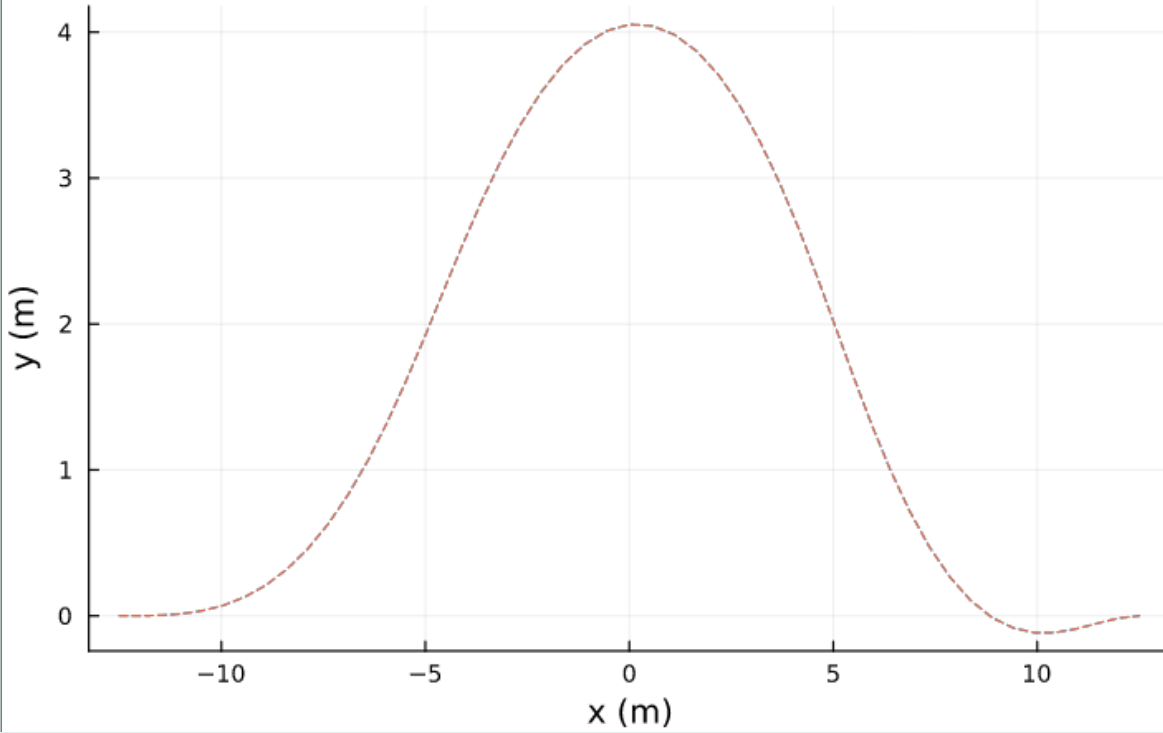
\includegraphics[width=0.5\linewidth]{trajectory}
        \caption{Simple parabolic trajectory for robot to follow}
        \label{fig:trajectory}
    \end{figure}

    \subsubsection{Metrics} \label{sec:results:metrics}
%    \textbf{TODO: Include metrics here, with references}
    Borrowing from the robotics field of odometry \cite{metrics1}, two metrics based off the absolute root-mean-square error (RMSE) were included to gauge how well the optimizer performed in trajectory optimization:
    \pagebreak
    
    \begin{itemize}
        \item Absolute Position RMSE: RMSE positional difference between calculated and reference trajectory at each point \begin{align*}
            \mathrm{RMSE}_{\mathrm{pos}} &= \transp{X - X_{ref}} * \mathrm{diag}\transbmat{1 & 1 & 0 & 0 & 0} * \left(X - X_{ref}\right) \fracln
            &= \sqrt{\strut \dfrac{1}{N} \sum^N_{k=1} \left[\left(p_{x,k} - p_{xref, k}\right)^2 + \left(p_{y,k} - p_{yref, k}\right)^2\right]  \strut\strut }
        \end{align*}
        \item Absolute Orientation RMSE: RMSE orientational difference between calculated and reference trajectory at each point\begin{align*}
            \mathrm{RMSE}_{\mathrm{orient}} &= \transp{X - X_{ref}} *  \mathrm{diag}\transbmat{0 & 0 & 1 & 0 & 0} * \left(X - X_{ref}\right) \fracln
            &= \sqrt{\strut \dfrac{1}{N} \sum^N_{k=1} \left(\theta_{k} - \theta_{ref, k}\right)^2 \strut\strut }
        \end{align*}
    \end{itemize}
    
    We also included the quadratic trajectory cost without regularization outlined in Section as a metric. It is mainly useful for debugging and comparing which trajectories were the hardest to optimize from a cost standpoint.

    \def\quadcost{\ensuremath{\mathcal{L}_Q}}
    \def\rmsepos{\ensuremath{\mathrm{RMSE}_{\mathrm{pos}}}}
    \def\rmseorient{\ensuremath{\mathrm{RMSE}_{\mathrm{orient}}}}

    \subsubsection{Baseline: No Control Input}
    We ran the tracker with no controller input (i.e. $P = D = 0$) as a baseline. The generated trajectory is shown in Figure \ref{fig:trajectorynocontrol} below.
    
    \begin{figure}[h!]
        \centering
        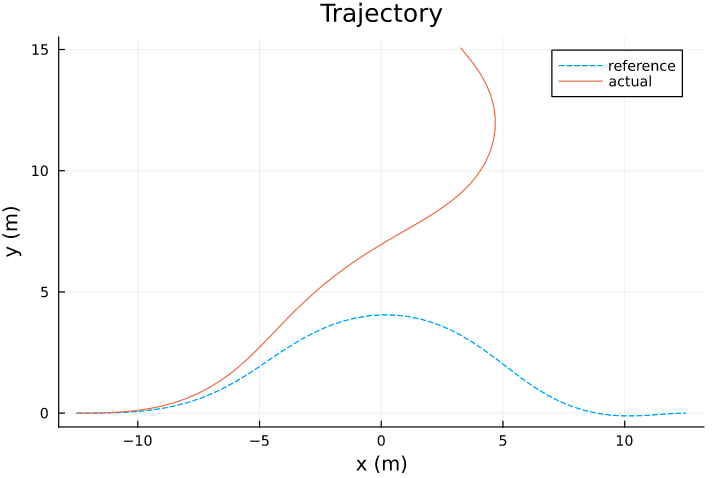
\includegraphics[width=0.55\linewidth]{img/trajectory_nocontrol}
        \caption{Generated trajectory without control ($ P = D = 0$)}
        \label{fig:trajectorynocontrol}
    \end{figure}

    \pagebreak
    
    \subsubsection{Without Regularization} \label{sec:results:singletraj:noreg}
    With the simple non-regularized quadratic cost, we found that our P/D matrices had very large values, and caused the optimizer to fail completely, with infinite values for all metrics. See Section \ref{sec:discussion:failurecase} for a discussion on potential failure reasons.
        \begin{align*}
            \hspace{-2em}
            P &= \bmat{-25.48 & -43.88 & 228.95 & 904.98 & 1151.69 \\
                -1.81 & -4.19 & 29.26 & -70.38 & -26.2} \fracln 
            D &
            = \bmat{-130.93 & -71.37 & -1142.36 & 22.02 & 2424.28 \\
                -9.39 & 10.48  & -19.01 & 3.23 & 186.85}
        \end{align*}
    
    \begin{figure}[h!]
        \centering
        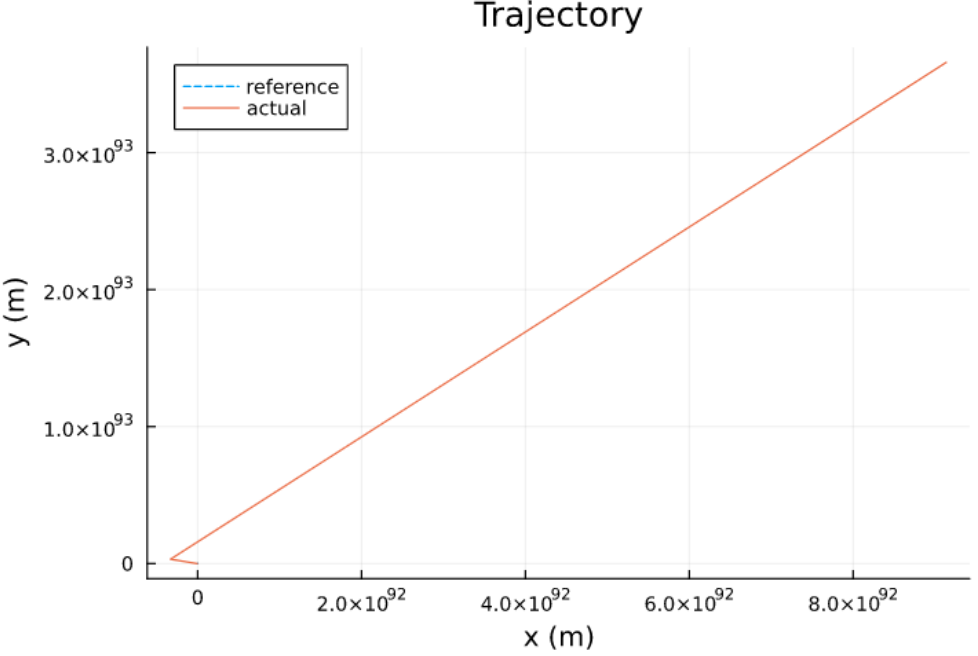
\includegraphics[width=0.6\linewidth]{img/trajectory_pd_noreg}
        \caption{Calculated trajectory with no regularization}
        \label{fig:trajectorypdnoreg}
    \end{figure}
    
    \pagebreak
    
    \subsubsection{With Regularization} \label{sec:results:singletraj:wreg}
    As can be seen in Figure \ref{fig:trajectorypdreg} below, regularization improves the generated trajectory signficantly and results in sparse $P $,$ D$ matrices with relatively small values, as expected from L1 regularization. 
        \begin{align*}
%            \hspace{-2em}
            P &= \bmat{-0.79 & 0.11 & 0 & 0 & 0 \\ -0.22 & -0.08 & 0 & 0 & 0} &
            D &= \bmat{-0.42 & 0 & 0 & 0 & 0 \\  0.2 & 0 & 0 & 0 & 0}
        \end{align*}
    
    \begin{figure}[h!]
        \centering
        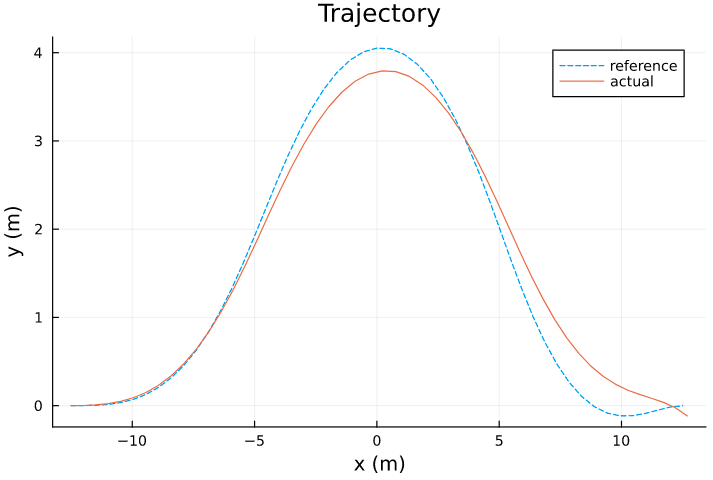
\includegraphics[width=0.6\linewidth]{img/trajectory_pd_reg}
        \caption{Generated trajectory with regularization}
        \label{fig:trajectorypdreg}
    \end{figure}
    
    \subsubsection{Metrics Comparison} \label{sec:results:singletraj:metrics}
    The metrics for the above cases are shown in Table \ref{tab:metrics:compare} below.
    \begin{table}[h!]
        \centering
        \tabvpad{1.5}
        \tabhpad{1.2em}
        \caption{Comparison of Metrics (rounded to 3 d.p.)} \label{tab:metrics:compare}
        \begin{tabular}{c|ccc}
            \hline
            & Baseline & With Reg. & \textit{Without Reg.}
            \\ \hline
            \rmsepos & 7.491 & 0.290 & $\infty$ \\
            \rmseorient & 0.976 & 0.060 & $\infty$ \\
            \quadcost & 314554.656 & 54.695  & $\infty$ \\
            \hline
        \end{tabular}
    \end{table}
    
    As evident from Table \ref{tab:metrics:compare} above, the generated PD matrix using our algorithm (with regularization) clearly improved all metrics. The metrics for the optimization without regularization were all reported to be infinity, and we attempt to discuss why in Section \ref{sec:discussion:failurecase} below.
    
    \section{Discussion} \label{sec:discussion}
    \subsection{Potential Reasons why Non-Regularized Quadratic Cost Failed} \label{sec:discussion:failurecase}
    
    \subsection{Effect of Regularization} \label{sec:discussion:regularization}
    
    \section{Learning Objectives} \label{sec:learningobjectives}
    In this project, we originally set out to learn more about optimal control and how optimization can be applied to the field. 
    This project was a indeed good opportunity (especially for Samuel who was more new to the field) to learn more about optimal control theory, particularly dynamics and trajectory optimization. A bigger part of our learning process involved trying to formulate our optimization problem, using what we learnt in class. Since dynamics-aware and trajectory-aware control problems can be quite complicated, it was challenging to do so in a way that was intuitive, while staying convex and easily solvable. Originally, we had wanted to autotune Q/R matrices for optimal control, but quickly found that the formulation was too complex; eventually, we simplified the problem by focusing on PID control and autotuning (optimizing for) P/D matrices. Still, formulating the optimization problem from scratch was not exactly non-trivial, but we used the techniques learnt in class to do it. In particular, we first tried a quadratic cost function with linear constraints to formulate a simple quadratic programming problem, and when that cause the values to explode, we turned to L1 regularization, which worked very well. 
    
    \bibliographystyle{ieeetr}
    \bibliography{cite.bib}
\end{document}

